\draft
\begin{parts}
	\part
	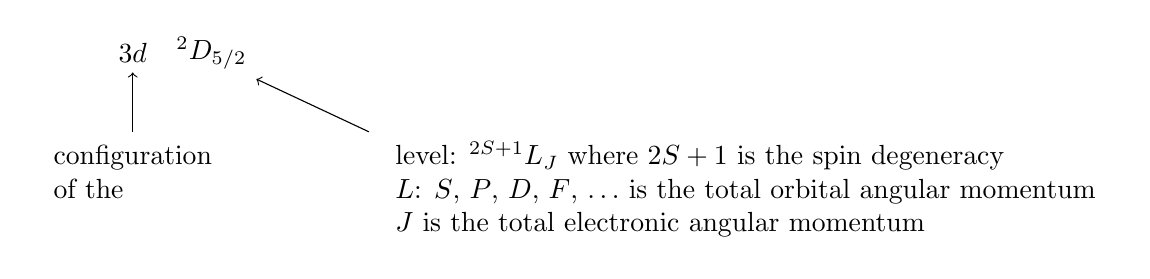
\begin{tikzpicture}[baseline=(config.base)] % Magic from https://tex.stackexchange.com/a/203881
		\node (config) at (0, 0) {$3d$};
		\node (level) at (1, 0) {${}^2 D_{5/2}$};
		\node [anchor=north] (config-text) at (0, -1) {
			\begin{tabular}{l}
			configuration\\
			of the $\electron$
			\end{tabular}
		};
		\node [anchor=north west] (level-text) at (3, -1) {
			\begin{tabular}{l}
			level: ${}^{2S+1} L_J$
			where $2S+1$ is the spin degeneracy\\
			$L$: $S$, $P$, $D$, $F$, $\ldots$ is the total orbital angular momentum\\
			$J$ is the total electronic angular momentum
			\end{tabular}
		};
		\path [draw, ->] (config-text.north)--(config.south);
		\path [draw, ->] (level-text.north west)--(level.south east);
	\end{tikzpicture}
	
	Large transition amplitude corresponds to the electric dipole transition, which has the following selection rules:
	
	\begin{gather*}
		\textnormal{Config}
		\begin{cases}
			\Delta n = \textnormal{any} \\
			\textnormal{1 $\electron$ transition} \\
			\Delta l = \pm 1
		\end{cases}
		\qquad
		\textnormal{Term}
		\begin{cases}
			\Delta L = 0, \pm 1 (0 \nrightarrow 0) \\
			\Delta S = 0
		\end{cases}
		\\[1em]
		\textnormal{Level}
		\begin{cases}
			\Delta J = 0, \pm 1 (0 \nrightarrow 0) \\
			\Delta M_J = 0, \pm 1 (0 \nrightarrow 0 \textnormal{ iff } \Delta J = 0)
		\end{cases}
	\end{gather*}
	
	Origin of electronic configuration:
	
	Recall that for a multi-$\electron$ atom,
	\begin{equation*}
		\hat{H} = \sum_i \sbracket{\dfrac{\hat{\mathbf{p}}_i^2}{2m_e} - \dfrac{Ze^2}{4\pi\permittivity\hat{r}_i} + \sum_{j>i}\dfrac{e^2}{4\pi\permittivity\hat{r}_{ij}}}
	\end{equation*}
	and by introducing a central field $S(r)$, we may write$\hat{H} = \hat{H}_\textnormal{CF} + \Delta\hat{H}_\textnormal{RE}$ where $\hat{H}_\textnormal{CF} = \sum_i \sbracket{\dfrac{\hat{\mathbf{p}}_i^2}{2m_e} - \dfrac{Ze^2}{4\pi\permittivity\hat{r}_i} + S(r_i)}$ and $\Delta\hat{H}_\textnormal{RE} = \sum_i \sbracket{-S(r_i) + \sum_{j>i}\dfrac{e^2}{4\pi\permittivity\hat{r}_{ij}}}$.
	The wavefunction of the atom may then be written as $\psi_{1s} + \psi_{2s} + \ldots$ and these are electronic configuration.
	
	\part \ion{Ca}{+} ground config by Aufbau principle: $1s^2 2s^2 2p^6 3s^2 3p^6 4s$
	
	$\Rightarrow$ $L=0$, $S=1/2$ $\Rightarrow$ Term: ${}^2 S$ $\Rightarrow$ Level: ${}^2 S_{1/2}$
	
	Try excited state $3d$, $L=2$, $S=1/2$ $\Rightarrow$ Term: ${}^2 D$ $\Rightarrow$ Levels: ${}^2 D_{3/2}$, ${}^2 D_{5/2}$
	
	$4p$ has term ${}^2 P$ $\Rightarrow$ Levels: ${}^2 P_{1/2}$, ${}^2 P_{3/2}$
	
	Recall the electric dipole selection rules above, we then have the following transitions:
	\begin{tikzpicture}[auto]
		\matrix (SP)[matrix of math nodes,row sep=1cm,column sep=16mm] {
			4s \;\; {}^2 S_{1/2} & 4p \;\; {}^2 P_{1/2} \\
			& {}^2 P_{3/2} \\
		};
		\draw (SP-1-1)--(SP-1-2);
		\draw (SP-1-1)--(SP-2-2);
	\end{tikzpicture}
	
	\begin{tikzpicture}[auto]
		\matrix (PD)[matrix of math nodes,row sep=1cm,column sep=16mm] {
			4p \;\; {}^2 P_{1/2} & 3d \;\; {}^2 D_{3/2} \\
			{}^2 P_{3/2} & {}^2 D_{5/2} \\
		};
		\draw (PD-1-1)--(PD-1-2);
		\draw (PD-2-1)--(PD-1-2);
		\draw (PD-2-1)--(PD-2-2);
	\end{tikzpicture}
	
	So the doublets are due to the transitions between levels.
	\image{.8\linewidth}{q1-transitions}
	The third line is due to the spin-orbit coupling that introduces fine structure splitting.
	
	\part For \SI{393.4}{\nano\metre} transition, we may observe $\pi$ and $\sigma$ radiation perpendicular to the field.
	\image{.3\linewidth}{q1-zeeman-transitions}
	So there should be 2 lines.
\end{parts}
